
\section{Geometry and the Steenrod squares} % <<<
\label{GeometryAndTheSteenrodSquares}
\ifx\OutputGeometryAndTheSteenrodSquares\undefined\else
Today begins a several days blitz on Steenrod operations, from a somewhat geometric point of view.
%  To begin, remember that reduced ordinary cohomology is representable:
%\[
%\widetilde H^q(X; \pi) = [X, K(\pi, q)].
%.\]
%\qquad\textup{For example:}\qquad
%\[
%\widetilde H^q (S^n;\pi) = \pi_n (K(\pi, q)) = \begin{cases}\pi & q = n, \\ 0 & q \ne n.\end{cases}
%\]

Fix from the beginning a subgroup $\pi$ of the symmetric group $\Sigma_n$ (we will mostly be concerned with the case $\pi = \Z_2=\Sigma_2$).
Consider the space $E\pi$, a contractible CW-complex with a free $\pi$-action, and the orbit space $B\pi=E\pi/\pi$. Fix a choice of $E\pi$ and a point $e\in E\pi$, and let $b\in B\pi$ be its image.

For example, if $\pi = \Z_2$, then $\pi$ acts antipodally on $S^{n-1}$.  $S^{n-1}$ is not contractible, but its image is contractible in $S^n$; that is, the inclusion $S^{n-1} \into S^n$ is null-homotopic.  So the direct limit of the inclusions $S^{n-1} \subset S^n \subset \cdots = \bigcup_n S^n = S^\infty$ is contractible and has a free $\pi$-action.  The orbit space $E\pi/\pi = B\pi$ is clearly seen to be $\RP^\infty$.


A basepoint $\ast$ in a space $X$ gives a lot more than you might think at first.  It induces, for example, a filtration of the $n$-fold product $X^n$, by defining:
\[
F_k X^n = \{(x_1, \ldots, x_k)\in X^n \mid \hbox{at most $k$ of the $x_i$ differ from $*$}\}
,\text{ so that:}\]
\begin{diagram}[height=1.3em]
F_0 X^n & \subseteq & F_1 X^n & \subseteq & \cdots & \subseteq & F_{n-1} X^n & \subseteq & F_n X^n \\
\uEqualto & & \uEqualto & & & & \uEqualto & & \uEqualto \\
\ptspace & & \bigvee_{i=1}^n X & & & & \hbox{``Fat wedge''} & & X^n
\end{diagram}
$\pi$ acts on $X^n$ by permuting the factors, and this action preserves the filtration.

Okay, so here's the key construction: on the universal $\pi$-bundle $E\pi \to B\pi$, use the Borel construction to mix in $X^n$; we thus obtain a locally trivial bundle over $B\pi$ with fiber $X^n$:
\begin{diagram}[height=1.7em]
X^n & \rTo & E\pi \times_\pi X^n \\
& & \dTo \\
& & B\pi
\end{diagram}
(Recall that $\pi$ acts diagonally on $E\pi \times X^n$, and $E\pi \times_\pi X^n$ is obtained as the quotient space of this action.)  This construction is called the ``$\pi$-extended power of $X$.''

Now the fact that the $\pi$-action on $X^n$ respects the filtration means that we have a sub-bundle
\begin{diagram}[height=1.7em]
E\pi \times_\pi F_{n-1}X^n & \subseteq & E\pi \times_\pi X^n \\
\dTo & & \dTo \\
B\pi & \rEqualto & B\pi
\end{diagram}
We want to pinch this subbundle to a point.  First, as $X^n / F_{n-1} X^n\cong X^{(n)}:=X\sprod\cdots\sprod X$, the $n$-fold smash product of $X$ with itself, we have:
\[
\frac{E\pi \times_\pi X^n}{E\pi \times_\pi F_{n-1} X^n} = \frac{E\pi \times_\pi X^{(n)}}{E\pi \times_\pi \ptspace}
.\]
This is almost the smash product, but $E\pi$ doesn't have a basepoint. Instead:%  But we can just add one in and then take the smash product, and this has no effect --- so
\[
\frac{E\pi \times_\pi X^n}{E\pi \times_\pi F_{n-1}X^n} = E\pi_+ \sprod_\pi X^{(n)}
,\]
where the symbol $\sprod_\pi$ means to take the orbit space of the diagonal action on $E\pi_+ \sprod X^{(n)},$ and $E\pi_+$ refers to $E\pi$ with a disjoint basepoint added.  This is called the ``$\pi$-adic construction'' on $X$ (for lack, really, of a better name), and will be written $D_\pi(X)$.

Now a map $f:X\to Y$ induces a map $D_\pi(X)\to D_\pi(Y)$, making $D_\pi$ into a functor.
Moreover, there is a map $i_X:X^{(n)}\to D_\pi(X)$ defined simply by $x\mapsto (e,x)$. Note that we can also describe $i_X$ in terms of the map $\overline{i_X}:X^n\to E\pi\times_\pi X^n$ defined by $x\mapsto(e,x)$. As $F_{n-1}X^n$ is mapped into $E\pi\times_\pi F_{n-1}X^n$, the map $\overline{i_X}$ descends to the quotient, and gives $i_X$:
\[i_X:X^{(n)}=\frac{X^n}{F_{n-1}X^n}\to \frac{E\pi \times_\pi X^n}{E\pi \times_\pi F_{n-1}X^n} = E\pi_+ \sprod_\pi X^{(n)}.\]

The maps $i_X$ constitute a natural transformation of functors $(\textup{---})^{(n)}\to D_\pi$, in the sense that for every $f:X\to Y$, there is a commuting diagram:
\[\xymatrix@R=6mm{
X^{(n)}\ar[r]_{f^{\wedge n}}\ar[d]_{i_X}&
Y^{(n)}\ar[d]^{i_Y}\\
D_\pi X\ar[r]^{D_\pi f}&
D_\pi Y
}
\]
For clarity, we list a number of functors and natural transformations that will soon be in use:
\begin{itemize}
\item $D_\pi(\DASH):\mathsf{Top}_*\to\mathsf{Top}_*$ as described above.
\item $(\textup{---})^{(n)}:\mathsf{Top}_*\to\mathsf{Top}_*$, the $n$-fold smash product.
\item $\widetilde H^*(\DASH):=\widetilde H^*(\textup{---};\F_p):\mathsf{Top}_*\to\mathsf{ComGrAlg}_{\F_p}$, ordinary reduced cohomology with coefficients in the field of $p$ elements, for some chosen prime $p$. This takes values in the category of (graded)-commutative graded $\F_p$-algebras.
\item $i_\DASH:(\DASH)^{(n)}\to D_\pi(\DASH)$, the natural transformation described above.
\item $(\DASH)^{\wedge n}:\widetilde H^r(\textup{---};\F_p)\to\widetilde H^{nr}((\DASH)^{(n)};\F_p)$, the $n$-fold smash power of a cohomology class.
\end{itemize}



The space $D_\pi Z$ is of some concern; first we want to know its cohomology.
\begin{lem}\label{lemaboutpiadic}
Suppose that $\widetilde H^i (Z) = 0$ for $i < q$, where coefficients are taken in a field $\F$, and that $\widetilde H^q (Z)$ is a finite dimensional $\F$-vector space.  Then,
\[\widetilde H^i(D_\pi Z)=
\begin{cases}0;&\textup{if }i<nq;\\(\widetilde H^q(Z)^{\otimes n})^\pi;&\textup{if }i=nq.%;\\???;&\textup{if }i>nq
\end{cases}
\]
Moreover, $i_Z^*:\widetilde H^{nq}(D_\pi Z)\to \widetilde H^{np}(Z^{(n)})$ is the inclusion of the $\pi$-invariants $(\widetilde H^q(Z)^{\otimes n})^\pi\subset\widetilde H^q(Z)^{\otimes n}$. Here, the tensor power is taken over $\F$, and $\pi$ acts thereupon by permuting factors.
\end{lem}
\begin{proof}
%One could produce a CW-complex for $D_\pi Z$ having no cells of dimension less than $nq$. No, one cannot! What if $Z$ is a $K(Z/3,d)$ and the field is $Z/2$? Then $H^*(Z;Z/2)=0$, but there's plenty of cells.
We have a map (drawn with dotted arrows) of bundle-subbundle pairs:
\[\xymatrix@!0@C=1.7cm@R=.8cm{
F_{n-1}Z^n\ar[dd]\ar[rd]\ar@{.>}[rr]&&F_{n-1}Z^n\ar'[d][dd]\ar[rd]\\
&Z^n\ar[dd]\ar@{.>}[rr]&&\ar[dd]Z^n\\
F_{n-1}Z^n\ar[dd]\ar[rd]\ar@{.>}'[r][rr]&&E\pi\times_\pi F_{n-1}Z^n\ar'[d][dd]\ar[rd]\\
&Z^n\ar[dd]\ar@{.>}[rr]&&\ar[dd]E\pi\times_\pi Z^n\\
\{b\}\ar@{.>}'[r][rr]\ar@{=}[rd]&&B\pi\ar@{=}[rd]\\
&\{b\}\ar@{.>}[rr]&&B\pi
}\]
Now the map $Z^{(n)}=\frac{Z^n}{F_{n-1}Z^n}\longrightarrow\frac{E\pi \times_\pi Z^n}{E\pi \times_\pi F_{n-1}Z^n} = D_\pi Z$ induced by this diagram is exactly $i_Z$, so we can study $i^*_Z$ using the associated morphism of relative Serre spectral sequences.

The relative Serre spectral sequence for the pair on the left has untwisted coefficients:
\[
_LE_2^{s,t} = H^s(*; H^t(Z^n, F_{n-1} Z^n)) \Rightarrow \widetilde H^{s+t}(Z^{(n)})
.\]
Now $B \pi$ is not simply connected (it is in fact a $K(\pi,1)$), so the second relative Serre spectral sequence will require twisted coefficients:
\[
_RE_2^{s,t} = H^s(B\pi; \{H^t(Z^n, F_{n-1} Z^n)\}) \Rightarrow \widetilde H^{s+t}(D_\pi Z)
.\]
Now $H^*(Z^n, F_{n-1} Z^n) \cong \widetilde H^* (Z^{(n)}) \cong \widetilde H^*(Z)^{\otimes n}$, and this last isomorphism is equivariant with respect to permutations, a fact that is not trivial (and likely to be false with other cohomology theories).  It follows that in both spectral sequences, everything is zero below the horizontal line at height $nq$ in the $E_2$ term. That is $E_2^{s,t}=0$ for $t<nq$.  So, % why?
\[
\widetilde H^{nq}(D_\pi Z) ={_RE_2^{0,nq}}= H^0(B\pi; \{\widetilde H^q(Z)^{\otimes n}\}) = (\widetilde H^q(Z)^{\otimes n})^\pi.\]
Moreover, the map $i^*_Z:\widetilde H^{nq}(D_\pi Z)\to \widetilde H^{nq}(Z^{(n)})$ coincides with the induced map $_RE_2^{0,nq}\to{_LE_2^{0,nq}}$, i.e.: % on the $E_2$ page. This is the map
\[H^0(B\pi; \{\widetilde H^q(Z)^{\otimes n}\})\to H^0(*;\widetilde H^q(Z)^{\otimes n}),\]
which is simply the inclusion of the $\pi$-invariants, as desired.
\end{proof}
\noindent This is the key fact that gives the Steenrod operations; all else follows more or less from it.

From here on, for all $r$, let $K_r$ denote $K(\Z_p,r)$ and $\widetilde H^r(\DASH)$ denote $\widetilde H^r(\textup{---};\Z_p)$, for some chosen prime $p$.  By the Hurewicz theorem and universal coefficients theorem: % rework this lecture so that we can swap out singular cohomology for something else.  this seems to be the key confusing step
\[\widetilde H^i(K_q)=0\text{ \ for $i<q$, and \ }\widetilde H^q(K_q)=\Z_p.\]
%%%$\widetilde H^i(K_q; \Z_2)$ is zero for $i<q$ and is $\Z_2$ when $i=q$.
%\begin{align*}
%\widetilde H^i(K_q; \Z_2) & = 0, \hspace{5em} i < q \\
%\widetilde H^q(K_q; \Z_2) & = \Z_2,
%\end{align*}
%by the Hurewicz theorem.
So $\widetilde H^{nq}(D_\pi K_q)$ is the $\pi$-invariants in $H^{nq}(K_q^{(n)})=(\Z_p)^{\otimes n}$ under the action of $\pi$ given by interchanging terms in the tensor product. However, this action is trivial.\footnote{In fact, the standard isomorphism $(\Z_p)^{\otimes n}\to\Z_p$ is $\Sigma_n$-equivariant, where we give the target the trivial action.}
% fa Moreover, as $\pi$ can only act trivially on $\widetilde H^{nq} (K_q^{(n)})=\Z_p$ \textbf{(is this true if $p\neq2$, or should we just set $p=2$ already?)},
Thus, the map
\[
\widetilde H^{nq} (D_\pi K_q) \xrightarrow{\ i^*\,} \widetilde H^{nq} (K_q^{(n)}) % this breaks if the action of pi isn't transitive
\]
is an isomorphism.  Now $\widetilde H^{nq} (K_q^{(n)})$ contains an element $\iota_q^{\sprod n}$, the $n$-fold smash power of the fundamental class $\iota_q \in \widetilde H^q( K_q)$, and we have shown:
\begin{cor}
There is a unique class $P_\pi \iota_q \in \widetilde H^{nq} (D_\pi K_q)$ such that $i^* P_\pi \iota_q = \iota_q^{\sprod n}$. That is, there is a unique pointed map $P_\pi\imath_q$ up to homotopy making the following diagram commute up to homotopy:
\[\xymatrix@R=6mm{
K_q^{(n)}\ar[d]^i\ar[r]^{\imath_q^{\sprod n}}&
K_{nq}\\
D_\pi K_q\ar@{.>}[ru]_{P_\pi\imath_q}
}\]
\end{cor}
\noindent Here, we have abused notationally the natural correspondence
$\widetilde H^q( X)  \longleftrightarrow [X, K_q]_\ast$ given by % \\
$f^* \iota_q  \longleftrightarrow [f]$ which holds for pointed spaces $X$.\footnote{For example: $\widetilde H^q (S^n;\pi) = \pi_n (K(\pi, q)) = \begin{cases}\pi & q = n, \\ 0 & q \ne n.\end{cases}$} We will continue to freely confuse these sets.

Now suppose that $X$ is any space (with no assumptions on its cohomology), and $u\in\widetilde H^q(X)$.
Representing $u\in \widetilde H^q(X)$ as a (homotopy class of) map(s) $u: X \to K_q$, we have a diagram:%n induced map $X^{(n)} \stackrel{u^{\sprod n}}{\to} K_q^{(n)} \stackrel{\iota_q^{\sprod n}}{\to} K_{nq}$, and then the diagram
\[\xymatrix@R=6mm{
X^{(n)}\ar[r]^{u^{\wedge n}}\ar[d]^i&
K_q^{(n)}\ar[d]^i\ar[r]^{\imath_q^{\wedge n}}&
K_{nq}\\
D_\pi X\ar[r]^{D_\pi u}&
D_\pi K_q\ar@{.>}[ru]_{P_\pi\imath_q}
}
\raisebox{-.5cm}{\textup{\qquad which induces:\qquad}}
\xymatrix@R=6mm{
\widetilde H^{nq}X^{(n)}&
\widetilde H^{nq}K_q^{(n)}\ar[l]_{(u^{\wedge n})^*}&
\widetilde H^{nq}K_{nq}\makebox[0cm][l]{$\,\ni\imath_{nq}$}
\ar@{.>}[dl]^{(P_\pi\imath_q)^*}\ar[l]_{(\imath_q^{\wedge n})^*}\\
\widetilde H^{nq}D_\pi X\ar[u]_{i^*}&
\widetilde H^{nq}D_\pi K_q\ar[l]_{(D_\pi u)^*}\ar[u]_{i^*}^\cong
}\phantom{\,\ni\imath_{nq}}\]
So we have a natural transformation $u\mapsto (D_\pi u)^* (P_\pi\imath_q)$ of functors $H^q(\textup{---};\F_p)\longrightarrow H^{nq}(D_\pi(\textup{---});\F_p)$.
As any cohomology class $u\in\widetilde H^q(X)$ can be written as $u^*(\imath_q)$, this discussion proves:
\begin{lem}
There is a unique natural transformation $P_\pi:H^q(\textup{---};\F_p)\longrightarrow H^{nq}(D_\pi(\textup{---});\F_p)$ such that $i_X^*P_\pi u=u^{\wedge n}$ for all $u\in H^q(X)$. $P_\pi u$ is called the \emph{``Steenrod power''} of $u$.
\end{lem}
%\begin{diagram}
%X^{(n)} & \rTo^{u^{\sprod n}} & K_q^{(n)} & \rTo^{\iota_q^{\sprod n}} & K_{nq}\\
%\dTo<p & & \dTo>p & \ruTo_{P_\pi \iota_q} \\
%D_\pi X & \rTo^{D_\pi u^{\sprod n}} & D_\pi K_q
%\end{diagram}
%induces a (\textbf{WRONG}) diagram on cohomology
%\begin{diagram}
%\widetilde H^{nq} X^{(n)} & \lTo^{(u^{\sprod n})^*} & \widetilde H^{nq} K_q^{(n)} & \lTo^{(\iota_q^{\sprod n})^*} & \widetilde H^{nq} K_{nq}\\
%\uTo<{p^*}>\cong & & \uTo>{p^*}<\cong & \ldTo_{(P_\pi \iota_q)^*} \\
%\widetilde H^{nq} D_\pi X & \lTo^{(D_\pi u^{\sprod n})^*} & \widetilde H^{nq} D_\pi K_q
%\end{diagram}
%which shows that there is a unique class $P_\pi u = P_\pi \iota_q \circ D_\pi u^{\sprod n} \in \widetilde H^{nq} D_\pi X$ such that $p^* P_\pi u = \iota_q^{\sprod n} \circ u^{\sprod n}$.
Finally, the diagonal map $\Delta: X \to X^{(n)}$ is equivariant, where we let $\pi$ act trivially on the single factor $X$, and this induces
\begin{diagram}[height=1.3em]
E\pi_+ \sprod_\pi X & \rTo^\Delta & E \pi_+ \sprod X^{(n)} \\
\dEqualto & & \dEqualto \\
B \pi_+ \sprod X & \rTo_j & D_\pi X.
\end{diagram}
So, any $u \in \widetilde H^q (X)$ gives us a class $j^* P_\pi u \in \widetilde H^{nq}(B \pi_+ \sprod X)$.

The case we will develop in full is $\pi = \Z_2$, $n = 2$, and $p=2$, so we specialise to this case now, writing $P$ for $P_\pi$ (and $\widetilde H^*(\DASH)$ for $\widetilde H^*(\DASH;\F_2)$). In this case, $B\pi = \RP^\infty$, and $H^*( B\pi) = \widetilde H^* (B\pi_+) = \Z_2[x]$ with $|x| = 1$. By the K\"unneth theorem, $\widetilde H^*(B\pi_+ \sprod X) \cong H^*(B \pi) \otimes \widetilde H^* (X)$, so given $u\in\widetilde H^q(X)$, we can write
%\begin{align*}
%\widetilde H^*(B \pi_+ \sprod X) & \cong H^*(B \pi) \otimes \widetilde H^* X \\
%j^* P u & = \sum_{i=-q}^q x^{q-i} \otimes \Sq^i u,
%\text{\qquad where $\Sq^iu\in
%\end{align*}
\[j^* P u  = \sum_{i=-q}^q x^{q-i} \otimes \Sq^i u,
\text{\qquad where }\Sq^iu\in \widetilde H^{q+i}(X).\]
We take this to be the \emph{definition} of $\Sq^i u$. We can note immediately that $\Sq^i$ is a natural transformation $\widetilde H^q\to\widetilde H^{q+i}$. Moreover, $\Sq^i u$ is zero when $-q\leq i<0$, since this holds in the universal case $K(\Z_2,q)$. (We will still allow ourselves to write $\Sq^iu$ for $i>q$, and define it to be zero).

Note that the above can be to a large extent carried out in other cohomology theories, giving similar operations.  Mostly one needs to have computed $\widetilde H^*(B \pi \sprod X)$.

Now let's start finding properties of the squares.  First of all, we don't even know that they're not all zero yet. Choose $u\in \widetilde H^q(X)$. There is a map $k:S^0\to B\pi_+$, where if $S^0=\{\pm1\}$, we set $k(1)=*$ and $k(-1)=b$. We have the following diagram
\[\xymatrix@R=.6cm{
B\pi_+ \sprod X \ar[r]^j & D_\pi X \\
S^0 \sprod X  \ar[r]^\Delta\ar[u]^{k\wedge 1} & X^{(2)}\ar[u]^i
}
\raisebox{-.5cm}{\textup{\qquad which induces:\qquad}}
\xymatrix@R=.6cm{
\sum_{i=0}^q x^{q-i} \otimes \Sq^i u\ar@{|->}[d]&
\ar@{|->}[l]  Pu \ar@{|->}[d]\\
u\smile u & u^{\wedge2}\ar@{|->}[l]
}\raisebox{-.5cm}{\textup{\qquad on $\widetilde H^{2q}(\DASH)$.\qquad}}
\]
Now $(k\wedge 1)^*: \Z_2[x]\otimes \widetilde H^* (X)\to\widetilde H^* (X)$ is the projection onto $\Z_2\otimes \widetilde H^* (X)$. Thus $\Sq^q u = u^2$.

Next, we derive the Cartan formula, using the following map $\delta:D_\pi(X\wedge Y)\to D_\pi(X)\wedge D_\pi(Y)$:
\begin{align*}
D_\pi(X \sprod Y) = E \pi_+ \sprod_\pi (X \sprod Y)^{(2)} & \stackrel{\delta}{\to} E \pi_+ \sprod_\pi X^{(2)} \sprod E \pi_+ \sprod_\pi Y^{(2)} = D_\pi X \sprod D_\pi Y, \\
(z, (x_1, y_1), (x_2, y_2)) & \mapsto (z, (x_1, x_2), z, (y_1, y_2)).
\end{align*}
Note that the following diagram commutes:
\begin{diagram}[height=1.8em]
(X \sprod Y)^{(2)} & \rTo^i & D_\pi(X \sprod Y) & \lTo^j & B \pi_+ \sprod (X \sprod Y) \\
\dTo<{T} & & \dTo>\delta & & \dTo>{\Delta_{B \pi_+}} \\
X^{(2)} \sprod Y^{(2)} & \rTo^{i \sprod i} & D_\pi X \sprod D_\pi Y & \lTo^{j \sprod j} & B \pi_+ \sprod X \sprod B \pi_+ \sprod Y
\end{diagram}
\begin{lem}
$\delta^*(Pu \sprod Pv) = P(u \sprod v)$.
\end{lem}
\begin{proof}
We can assume $X = K(\pi, p)$, $Y = K(\pi, q)$, $u = \iota_p$, and $v = \iota_q$.  Then the lowest dimensional cohomology of $X \sprod Y$ is $\Z_2$ in dimension $(p + q)$. Thus $i:(X\wedge Y)^{(2)}\to D_\pi(X\wedge Y)$ induces a monomorphism on $H^{2(p+q)}$, by lemma \ref{lemaboutpiadic}. Now in the diagram:
\[\xymatrix@R=.6cm{
H^{2(p+q)}((X\wedge Y)^{(2)})&H^{2(p+q)}(D_\pi(X\wedge Y))\ar@{_{(}->}[l]_{i^*}\\
H^{2(p+q)}(X^{(2)}\wedge Y^{(2)})\ar[u]^{T^*}&H^{2(p+q)}(D_\pi X\wedge D_\pi Y)\ar[l]_{(i\wedge i)^*}\ar[u]^{\delta^*}
}\raisebox{-.5cm}{\textup{\qquad we know:\qquad}}
\xymatrix@R=.6cm{
(\imath_p\wedge \imath_q)^{(2)}&
\ar@{|->}[l]  P(\imath_p\wedge\imath_q)\\
\imath_p^{(2)}\wedge \imath_q^{(2)} \ar@{|->}[u]& P(\imath_p)\wedge P(\imath_q)\ar@{|->}[l]%\ar@{|->}[u]
}
\]
In particular, as $i^*$ is a monomorphism, $\delta^*(P(\imath_p)\wedge P(\imath_q))$ must equal $P(\imath_p\wedge\imath_q)$.
%  But $(\delta i)^*(P\iota_p \sprod P\iota_q) = ((i \sprod i)T)^* (\iota_p \sprod \iota_q)$ equals $(\iota_p \sprod \iota_q)^{\sprod 2}$, and $P(\iota_p \sprod \iota_q)$ is defined to be the unique class in $H^{2(p+q)} D_\pi(X \sprod Y)$ for which this holds. % we have two nonzero things living in the same dimension, where there's only one nonzero element.
\end{proof}

\begin{cor}[Cartan formula]  $\Sq^k(u \sprod v) = \sum_{i+j = k} \Sq^i u \sprod \Sq^j v$.
\end{cor}
\begin{proof} Almost immediate from the construction:
\begin{align*}
\sum_k x^{p+q-k} \otimes \Sq^k(u \sprod v) & = j^* P(u \sprod v) \\
& = j^* \delta^*(Pu \sprod Pv) \\
& = \Delta_{B \pi_+}^* (j \sprod j)^*(Pu \sprod Pv) \\
& = \Delta_{B \pi_+}^*\left[\left(\sum_i x^{p-i} \otimes \Sq^i u\right) \sprod \left(\sum_j x^{q-j} \otimes \Sq^j v\right)\right] \\ % be careful about mixing smash products and tensor products.  this happened earlier too.
& = \sum_{i, j}x^{p+q-i-j} \otimes \Sq^i u \sprod \Sq^j v.\qedhere
\end{align*}
\end{proof}
\noindent
Taking $X = Y$ and using $\Delta: X \to X \wedge X$, we obtain:
\begin{cor}[Internal version]  $\Sq^k(uv) = \sum_{i+j=k} \Sq^i u \Sq^j v$.
\end{cor}
\noindent In particular, it will be convenient to define the total squaring operation $\Sq:\widetilde H^*(X)\to\widetilde H^*(X)$, defined by $ u\mapsto\sum_i \Sq^i u$. The Cartan formula states precisely that $\Sq$ is a ring homomorphism.

\begin{lem}
If $e$ is the generator of $\widetilde H^1 (S^1) = \Z_2$ then $\Sq^0 e = e$.
\end{lem}

\begin{proof}
We know that $\Sq^i e = 0$ for $i>0$ since $H^{1+i}(S^1)=0$, so $j^*(P_{\pi}e)=x\Sq^0 e \in H^*(B\pi_+ \smash S^1)=\Z_2[x]\tensor H^*(S^1)$. Now $D_{\pi}S^1 = S^{\infty}_+\smash_{\pi} S^2$, where $\pi$ acts on $S^2$ by swapping the two factors. We can decompose $S^2$ as the smash product of the diagonal, which is a $\pi$-invariant $S^1_1$, and the antidiagonal $S^1_{-1}$ where $\pi$ acts by a reflection. Thus $D_{\pi}S^1=S^{\infty}_+\smash_\pi (S^1_1\smash S^1_{-1}) = (S^{\infty}_+\smash_{\pi}S^1_{-1})\smash S^1_1=\Sigma \RP^{\infty}$. Now $B\pi_+\smash S^1=\Sigma \RP^{\infty}$ too, and $j$ sends the $S^1$ factor into the diagonal $S^1_1$ by the identity map, so $j$ is the suspension of some map $\RP^{\infty}\to\RP^{\infty}$. This map comes from the map $S^{\infty}\to S^{\infty}\smash S^1$ including the $S^{\infty}$ into the $S^{\infty}$ factor by the identity map. Thus, it sends $[x_0,x_1,\ldots]\mapsto [0,x_0,x_1,\ldots]$. Since this map is homotopic to the identity, so is $j$ and hence $j^*$ is the identity map, and so since $P_\pi e\neq 0$, neither is $j^*P_{\pi}e$, which implies that $Sq^0e\neq 0$ so the only other option is that $\Sq^0 e = e$.
\end{proof}

% >>>
\fi
\BoxedNote{
\Bullet Fix $u\in\widetilde H^q(X)$. We summarise
% The following diagrams summarise
the construction of $\Sq^iu\in \widetilde H^{q+i}(X)$ thus:
\[\xymatrix@R=3mm@C=5mm{
B\pi_+\wedge X\ar[r]_j&D_\pi(X)&**[l]{X^{\wedge2}}\ar[l]^{\ \ \ i}\\
E\pi_+\wedge_\pi X\ar[r]^\Delta\ar@{=}[u]&
E\pi_+\wedge_\pi X^{(2)}\ar@{=}[u]
}
%\raisebox{-.3cm}{\textup{induces:\ }}
\raisebox{-.3cm}{\textup{on $\widetilde H^{2q}$:\ }}
\xymatrix@R=3mm@C=5mm{
%\sum x^{q-i}\otimes \Sq^iu
\text{\raisebox{-.05em}{$\Sigma$}\,{\small$x^{q-i}\otimes \Sq^iu$}}
&Pu\ar@{|->}[r]_{i^*}\ar@{|->}[l]^{\qquad\ \ j^*}&u\wedge u\\
&u\raisebox{0mm}[0cm][0cm]{\makebox[0mm][l]{$\,\in\widetilde H^q(X)$}\ar@{|->}[u]}
}
\]
\Bullet $\Sq^iu=0$ for $i<0$ and $i>q$. $\Sq^qu=u^2$.

\Bullet Internal Cartan formula: $\Sq^k(uv) = \sum_{i+j=k} \Sq^i u \Sq^j v$. In particular, the total squaring operation $\Sq$ defined by $ u\mapsto\sum_i \Sq^i u$ is a ring homomorphism.

\Bullet External Cartan formula: $\Sq^k(u \sprod v) = \sum_{i+j = k} \Sq^i u \sprod \Sq^j v$.
}
% THERE IS A LOT LEFT TO REPAIR IN THIS CHAPTER!
\section{Properties of the squares} % <<<
\label{PropertiesOfTheSquares}
\ifx\OutputPropertiesOfTheSquares\undefined\else
%\textbf{Perhaps we should simply delete everything in small caps.} I haven't edited what's here, since I'm not sure if it's needed. Also, I haven't thought through what's needed for this to generalise to an arbitrary field. Comments about that question might prefer to live in the previous lecture. Also, it would almost certainly be better to merge this lecture with the previous.
%
%\textsc{
%We continue to derive properties of the Steenrod squares.  Recall that by choosing $\pi \subseteq \Sigma_n$ and a space $X$ we get a space $D_\pi X = E \pi_+ \sprod_\pi X^{(n)}$ along with inclusions
%\begin{diagram}[height=2em]
%B\pi_+ \sprod X & \rTo^j & E\pi_+ \sprod_\pi X^{(n)} & \rEqualto & D_\pi X \\
%& & \uTo>p \\
%& & X^{(n)}.
%\end{diagram}
%Working with field coefficients, we found there was a unique natural transformation $P_\pi: \widetilde H^q X \to \widetilde H^{nq} D_\pi X$ such that
%\[
%p^* P_\pi u = u^{\sprod n}
%\]
%for all $u \in \widetilde H^q X$.  In the case that $\pi = \Z_2$, $n = 2$, we use the K\"unneth isomorphism $\widetilde H^* (B \pi_+ \sprod X) \cong \widetilde H^*B \pi_+ \otimes \widetilde H^* X$ and the fact that $\widetilde H^* B \pi_+ = H^*B \pi = \Z_2[x]$ to write for each $u \in \widetilde H^qX$,
%\[
%j^* P_\pi u = \sum_{i=0}^q x^{q-i} \otimes \Sq^i u \in \widetilde H^*(B \pi_+ \sprod X)
%.\]
%This characterizes $\Sq^i u$.  Since $P_\pi u \in \widetilde H^* D_\pi X$ has degree $2q$ and $x \in \widetilde H^* B\pi$ has degree $1$, $\Sq^i u \in \widetilde H^* X$ has degree $q + i$.}
%
%\textsc{
%These properties of $\Sq^i$ are immediate or were shown previously:
%\begin{itemize}
%\item $\Sq^i$ is a natural transformation of functors $\widetilde H^* \to \widetilde H^{*+i}$.
%\item $\Sq^i u = 0$ for $i > q$, $u \in \widetilde H^q X$.
%\item $\Sq^q u = u^2$ for $u \in \widetilde H^q X$.
%\item (Cartan formula) $\Sq^k(uv) = \sum_{i+j=k} \Sq^i u \Sq^j v$.
%\end{itemize}
%}

It was an exercise to show that $\Sq^0 e = e$, where $e$ is the generator of $\widetilde H^1 (S^1)$.  This important fact has several consequences.
\begin{cor}
$\Sq^k$ commutes with the suspension homomorphism $\sigma: \widetilde H^q (X) \to \widetilde H^{q+1} (\Sigma X)$.  We say that $\Sq^k$ is a ``stable operation.''
\end{cor}
\begin{proof}
The suspension homomorphism $\sigma$ is the composite
$\widetilde H^q (X)=\widetilde H^q (X)\otimes\widetilde H^1(S^1)\xrightarrow{\ \wedge e\ }\widetilde H^{q+1} (\Sigma X)$, and we calculate: $\Sq^k(\sigma u) = \Sq^k(u \sprod e) = \Sq^k u \sprod \Sq^0 e = \sigma \Sq^k u$.
\end{proof}
\begin{cor}
$\Sq^0: \widetilde H^q (X) \to \widetilde H^q (X)$ is the identity.
\end{cor}
\begin{proof}
It suffices to check this on the class $\iota_q \in \widetilde H^q(K_q)$, writing $K_q = K(\Z_2, q)$. Now $\Sq^0$ leaves the unique generator $e^{\sprod q} \in \widetilde H^q (S^q)$ fixed, by the Cartan formula. As the map $S^q\to K_q$ classifying $e^{\sprod q}$ induces an isomorphism $\widetilde H^q(K_q)\to \widetilde H^q(S^q)$, $\Sq^0$ fixes $\imath_q$.
%
% For $q = 1$, $\Sq^0 \iota_1 \ne 0$ because this is the universal case and the exercise showed that $\Sq^0\imath_1$ pulls back to the nontrivial class $e$ on $S^1$.  But $\widetilde H^1 K_1 = \Z_2$, so $\Sq^0$ is the identity on $\iota_1$.  Furthermore, $\Sq^0$ leaves $e^{\sprod q} \in \widetilde H^q S^q$ undisturbed, by an application of the Cartan formula and the fact that the squares commute with suspensions.  It follows that $\Sq^0 \iota_q = \iota_q$.
\end{proof}

\begin{fact}
The map $\beta: \widetilde H^q (X;\F_2) \to \widetilde H^{q+1} (X;\F_2)$ given by
\begin{diagram}[height=2em]
\widetilde H^q (X;\F_2) & \rTo^\beta & \widetilde H^{q+1} (X;\F_2) \\
\dTo<\delta & \ruTo_{\mathrm{reduction}} \\
\widetilde H^{q+1}(X; \Z),
\end{diagram}
where $\delta$ is the zigzag map of the coefficient sequence $0 \to \Z \stackrel{\cdot 2}{\to} \Z \to \Z_2 \to 0$ is called the Bockstein homomorphism.  It is $\Sq^1$.
\end{fact}

\begin{lem}
$\Sq^k$ is a group homomorphism.
\end{lem}
\begin{proof}
This holds for any stable cohomology operation.
%Using the correspondence $\widetilde H^nX=[X,K(n,\Z_2)]$, and applying
Representing cohomology classes by maps into Eilenberg-MacLane spaces, and using the naturality of $\Sq^k$, for any $u\in \widetilde H^q(X)$, we have a homotopy commuting diagram:
\[\xymatrix@C=1.75cm@R=7mm{
K_q\ar[r]^{\Sq^k\imath_q}&K_{q+k}\\
X\ar[u]^u\ar[ru]_{\Sq^ku}
}\]
That $\Sq^k$ commutes with suspension in this context means that the left hand diagram commutes. Taking adjoints, the right hand diagram commutes:
\[\xymatrix@C=1.75cm@R=.7cm{
\Sigma K_q \ar[d]^\sigma\ar[r]^{\Sigma \Sq^k \iota_q} & \Sigma K_{q+k} \ar[d]^\sigma\\
K_{q+1}  \ar[r]^{\Sq^k \iota_{q+1}} & K_{q+k+1}
}
\qquad\qquad
\xymatrix@C=1.75cm@R=.7cm{
K_q \ar[d]^\simeq\ar[r]^{\Sq^k \iota_q} &K_{q+k} \ar[d]^\simeq\\
\Omega K_{q+1}  \ar[r]^{\Omega\Sq^k \iota_{q+1}} & \Omega K_{q+k+1}
}\]
so $\Sq^k\imath_q$ is an $H$-space map (or an $H$-map).  The $H$-space structure on $K_q$ represents the addition on $\widetilde H^q$, so it follows that $\Sq^k$ is a homomorphism.
\end{proof}






% >>>
\fi
\BoxedNote{\Bullet $\Sq^k$ is stable --- it commutes with suspension; it is thus a homomorphism.

\Bullet $\Sq^0$ is the identity, $\Sq^1$ is the Bockstein.}
\section{The Adem relations} % <<<
\label{TheAdemRelations}
\ifx\OutputTheAdemRelations\undefined\else




The last basic fact about the squares is the Adem relations, for which we will take an approach using generating functions in the indeterminate $x$, following Bullett-MacDonald~\cite{BullettMacDonald}.  First, for $u \in \widetilde H^q X$ define $\Sq_x u = \sum x^{-k} \Sq^k u$, where $|x| = 1$ so that $\Sq_x$ is homogenous of degree 0.  For example, if $u \in \widetilde H^1(X)$, $\Sq_x u = u + x^{-1} u^2 = u^2(u^{-1} + x^{-1})$.  This $\Sq_x$ occurs naturally in the above as $j^* P u = x^q \Sq_x u.$  Also, $\Sq_x$ has the nice property that it is a ring homomorphism, as shown by the Cartan formula.

Second, take $\Sigma_4$ to be the symmetric group acting on four letters, arrange the letters into a square, and let $\omega$ be the subgroup of permutations which preserves the rows or transposes them, along with permutations within each row.\footnote{The group $\omega$ is sometimes called the ``wreath product'' $\pi \wr \pi$; it is in fact $D_8$, the $2$-Sylow subgroup of $\Sigma_4$.} That is, the subgroup generated by the three permutations, $\alpha,\beta,\gamma$:
\[
\newcommand{\DRAWPERM}[5]
{\left(\begin{array}{cc}a&b\\c&d\end{array}\xrightarrow{\ #5\ }
\begin{array}{cc}#1&#2\\#3&#4\end{array}\right)}
\DRAWPERM{b}{a}{c}{d}{\alpha},\qquad
\DRAWPERM{a}{b}{d}{c}{\beta},\qquad
\DRAWPERM{c}{d}{a}{b}{\gamma}.
\]
Now let $N=\langle\alpha,\beta\rangle$ be the subgroup of permutations preserving the rows, and let $H=\langle \gamma\rangle$ be the subgroup whose only nontrivial element swaps the two rows. Then $\omega$ is the semidirect product $N \rtimes H$. Note that $H$ acts from the left on $N$ via $h\cdot n=hnh^{-1}$. Let $\pi$ be the group $\{\pm1\}$ under multiplication. Then $N=\pi^2$ and $H=\pi$, and the action of $\pi$ on $\pi^2$ is by interchanging factors.

As $\omega=N \rtimes H$, an $\omega$-space is just an $H$-space with an $H$-equivariant $N$-action:
\begin{diagram}[height=1em]
N \times X & \rTo & X &&&&\pi^2 \times X & \rTo & X \\
\circlearrowright & & \circlearrowright &&\textup{i.e.}&&\circlearrowright & & \circlearrowright \\
H & & H&&&&
\pi & & \pi
\end{diagram}
%Now, what is an $\omega$-space $X$?  $X$ is a $\pi$-space with a $\pi$-equivariant $\pi^2$ action; i.e., we have
%\begin{diagram}[height=1em]
%\pi^2 \times X & \rTo & X \\
%\circlearrowright & & \circlearrowright \\
%\pi & & \pi,
%\end{diagram}
where the action of $\pi$ on $\pi^2\times X$ (i.e.\ $H$ on $N$) is the diagonal action.  An example of an $\omega$-space is $E \pi \times (E \pi)^2$. We view $E\pi$ as $S^\infty$ equipped with the antipodal map $a\mapsto-a$, so that the action of $\pi$ on $E_\pi$ can be written simply as $(\pm1,a)\mapsto\pm a$. The $\pi^2$ action is on the right-hand factor, with
%\[(x, y) \cdot (a, b, c) = (a, x \cdot b, y \cdot c),\]
\[((\pm1,\pm'1),(a,b,c))\mapsto(a, \pm b, \pm' c),\]
% and $\pi$ acting on $E \pi \times (E \pi)^2)$,
and the $\pi$ action is diagonal, acting as usual on the first factor, and by interchanging factors in the second:
\[(-1, (a, b, c)) = (-a, c, b).\]  The total space is contractible and its $\omega$-action is free; hence it is an $E \omega$, and we compute % should this section actually be (a, b, c) = (-a, -c, -b)?  Does it matter?  we already quotiented by the pi action on E pi...  plus, the original text reads "acting... by the antipodal map crossed with an exchange of factors in (E pi )^2."
\begin{align*}
B \omega & = (E \pi \times (E \pi)^2) / \omega \\
& = (E \pi \times (B \pi)^2) / \pi \\
& = E \pi \times_\pi (B \pi)^2.
\end{align*}

On one hand, giving a space $X$ a basepoint, we can do the $\omega$-adic construction
\[
D_\omega X = E \omega_+ \sprod_\omega X^{(4)} = \frac{E \omega \times_\omega X^4}{E \omega \times_\omega F_3 X^4}
.\]
However, we calculate:
\begin{align*}
E\omega\times_\omega X^4&=E\pi\times(E\pi)^2\times X^4/\omega\\
&=E\pi\times(E\pi\times_\pi X^2)^2/\pi\\
&=E\pi\times_\pi(E\pi\times_\pi X^2)^2
\end{align*}
Thus, the $\omega$-reduced power operation on $X$ is the iteration of the $\pi$-reduced power operation on $X$.  All this goes to show that $D_\omega X = E \omega_+ \sprod_\omega X^{(4)} = D_\pi(D_\pi X)$, so we have iterated the $\pi$-adic construction!  That ought to be a good thing, because the Adem relations concern iterated Steenrod operations.

Now we have a diagram commuting up to homotopy, where the map $\xi$ is induced by the inclusion $\pi^2\to\omega$:
\[\xymatrix@R=7mm@C=.5cm{
(X^{(2)})^{(2)} \ar[d]_i\ar@{=}[rr]&& X^{(4)} \ar[d]^i\\
D_\pi(D_\pi X) \ar[rr]^\cong && D_\omega X \\
D_\pi(B \pi_+ \sprod X) \ar[u]^{D_\pi j}
&B \pi_+ \sprod B \pi_+ \sprod X\ar[dr]_{\xi\sprod1}\\
B \pi_+ \sprod B \pi_+ \sprod X \ar[u]^j\ar[rr]^{\xi\wedge1}
\ar[ur]_{T\wedge1}&& B \omega_+ \sprod X\ar[uu]_j
%&B \pi_+ \sprod B \pi_+ \sprod X.\ar[ul]^{T\sprod1}\ar[ur]
}\]
The bottom triangle commutes up to homotopy because the flip map $T$ in% the diagram of exact sequences
\[\xymatrix@R=1mm{
\pi\times\pi\ar[dd]^T\ar[rd]\\
&\omega\ar[r]&\pi\makebox[0cm][l]{$\,\ni t$}\\
\pi\times\pi\ar[ru]
}\]
is induced by conjugation by the image of the nontrivial element $t$ of the right-hand $\pi$, and it is a basic fact about classifying spaces that a conjugation map $c_t: \omega \to \omega$ induces a map $B c_t: B \omega \to B \omega$ which is homotopic to the identity (essentially, $c_t$ moves the basepoint). % is this right?  i don't think this is homotopic to the identity
So in some sense the whole point of $\omega$ was to convert the outer automorphism $T: \pi \times \pi \to \pi \times \pi$ to an inner automorphism.  It follows that the map $D_\pi j \circ j: B\pi_+ \sprod B\pi_+ \sprod X \to D_\pi(D_\pi X)$ is $\pi$-equivariant up to homotopy.

Now if $u \in \widetilde H^q (X)$, we have
\begin{diagram}[width=2em,height=1.4em]
P_\omega u & \in & \widetilde H^{4q}(D_\omega X) \\
\dEqualto & & \dEqualto \\
P(Pu) & \in & \raisebox{0cm}[0cm][0cm]{\,$\widetilde H^{4q}$}(D_\pi D_\pi X).
\end{diagram}
Now $(D_\pi j \circ j)^* P(P u) \in \widetilde H^*(B\pi_+ \sprod B\pi_+ \sprod X) \cong \Z_2[x, y] \otimes \widetilde H^* (X)$, and the $\pi$-equivariance up to homotopy above means that this class is symmetric in $x$ and $y$.  So,
\begin{alignat*}{2}
(D_\pi j \circ j)^* P(P u) & = j^* P(j^* P u)&\qquad&\text{(naturality of $P$)} \\ % disambiguate those js
& = j^* P(y^q \Sq_y u) \\
& = x^{2q} \Sq_x(y^q \Sq_y u) \\
& = x^{2q} \Sq_x(y^q) \Sq_x \Sq_y u &&\text{($\Sq_x$ is a ring hom)} \\
& = x^{2q} y^{2q} (x^{-1} + y^{-1})^q \Sq_x \Sq_y u
\end{alignat*}
is symmetric in $x$ and $y$.  This is the shortest statement of the Adem relations.

We have shown that $\Sq_x \Sq_y u = \Sq_y \Sq_x u$, where $\Sq_x = \sum_{i \ge 0} x^{-i} \Sq^i$, and $|x| = |y| = 1$, and $x$ and $y$ represent $1$-dimensional classes in $\widetilde H^* (\RP^\infty)$, and now should derive from this the more standard form of the Adem relations. To begin, as $\Sq_x$ is a ring homomorphism,
\begin{align*}
\Sq_x \Sq_y & = \Sq_x \left( \sum_{j \ge 0} y^{-j} \Sq^j \right) \\
& = \sum_{j \ge 0}(\Sq_x y)^{-j} \Sq_x \Sq^j \\
& = \sum_{j \ge 0} y^{-2j}(x^{-1} + y^{-1})^{-j} \Sq_x \Sq^j.
\end{align*}
Now these coefficients are a mess, so, taking a lesson from calculus, we make a variable substitution, defining $t = y^{-2}(y^{-1} + x^{-1})^{-1}$.  So $|t| = -1$, and now
\begin{align*}
\Sq_x \Sq_y & = \sum_{j \ge 0} t^j \Sq_x \Sq^j \\
& = \sum_{j \ge 0} t^j \sum_{i \ge 0} x^{-1} \Sq^i \Sq^j \\
& = \sum_{i, j \ge 0} t^j x^{-i} \Sq^i \Sq^j.
\end{align*}
Letting $s = x^{-1}$, so $|s| = -1$, we have $\Sq_x \Sq_y = \sum_{i, j \ge 0} s^i t^j \Sq^i \Sq^j$, a generating function for products of squares.  On the other hand,
\begin{align*}
\Sq_y \Sq_x & = \sum_{j \ge 0}(\Sq_y x)^{-j} \Sq_y \Sq^j \\
& = \sum_{i, j \ge 0} x^{-2j} y^{2j} t^j y^{-i} \Sq^i \Sq^j \\
& = \sum_{i, j \ge 0} s^{2j} t^j y^{2j-i} \Sq^i \Sq^j.
\end{align*}
We thus need to know how to express $y$ in terms of $t$ and $s$.

Now, $t^{-1} = y^2(x^{-1} + y^{-1}) = y + x^{-1} y^2 = y + s y^2$.  At this point we could pull out the quadratic formula, but that seems ill-advised over $\Z_2$.  Instead, we use the theory of residues: if $f(z)$ is a power series, then the coefficient of $z^m$ in $f(z)$ is the residue of $\frac{f(z)}{z^{m+1}}dz$.  (Normally there's a factor of $2 \pi i$ or something floating around, but once again this seems ill-advised in $\Z_2$.)  Now we are going to take advantage of the $dz$ to change variables and the claim is that this works for power series over any ring.\footnote{This is nearly true, nearly false.  It does work in this case.  See note at the end of this lecture \textbf{(what note?)}. % ... what note?
}  So in our case, we take the coefficient of $(t^{-1})^k$ in $y^m$: \[\res \frac{y^m}{(t^{-1})^{k+1}} d(t^{-1}).\]  We calculate that $d(t^{-1}) = dy + sdy^2 = dy + 2sydy = dy$ (as we're working in $\Z_2$).  We then have
\[\res \frac{y^m dy}{y^{k+1}(1 + sy)^{k+1}} = \res \frac{(1+sy)^{-k-1} dy}{y^{k-m+1}},\]
which is equal to the coefficient of $y^{k-m}$ in $(1+sy)^{-k-1}$. That is $\binom{-k-1}{k-m}s^{k-m}$, where we simply agree that $(1 + z)^m = \sum \binom{m}{k} z^k$ for $m \in \Z$, and for $k < 0$, $\binom{m}{k} = 0$.

We now know what $y$ is in terms of $s$ and $t$, provided we know what the binomial coefficients are:
\[
y^m = \sum_{k \ge m} \binom{-k-1}{k-m} s^{k-m} t^{-k}\text{, \ so that}
\]
\[
\Sq_y \Sq_x = \sum_{i, j \ge 0} s^{2j} t^j y^{2j-i} \Sq^i \Sq^j = \mathop{\sum_{i, j \ge 0}}_{k\geq2j-1} \binom{-k-1}{k-2j+i} s^{k+i}t^{j-k}\Sq^i\Sq^j
.\]
Note that we could have specified that $ $ is the most recent sum, but if $k<2j-1$ then the binomial coefficient is zero anyway.
Now, in $\Sq_x \Sq_y$, the coefficient of $s^a t^b$ is $\Sq^a \Sq^b$.  In the most recent expression for $\Sq_y \Sq_x$, this term occurs when $k + i = a$ and $j - k = b$ --- viewing $j$ as the independent variable, we have $k = j - b$ and $i = a - k = a - j + b$.  We finally obtain:
\[
\Sq^a \Sq^b = \sum_{j=0}^{\lfloor a/2\rfloor} \binom{b-j-1}{a-2j} \Sq^{a+b-j} \Sq^j
,\]
and this last formula is called the ``Adem relation.''  One thing to notice is that if $a \le 2b$, then since $a \ge 2j$ we have $b \ge j$, so $a + b -j \ge 2j$.  So these relations let you express $\Sq^a \Sq^b$ for $a \le 2b$ as a sum of $\Sq^i \Sq^j$, where $i \ge 2j$.  Such $\Sq^i \Sq^j$ are called \emph{admissable}.

So the tensor algebra on the squares $T(\Sq^1, \Sq^2, \ldots)$ modulo the Adem relations acts on $H^*(X; \Z_2)$.  This algebra $T(\Sq^1, \ldots) / \{\hbox{Adem relations}\}$ is called the ``Steenrod algebra.''  It is denoted $\SA$.
\begin{lem}
$\SA$ is generated by $\Sq^{2^i}$, and these are exactly the indecomposables amoungst the generators $\{\Sq^1,\Sq^2,\Sq^3,\ldots\}$.
\end{lem}
\begin{proof}
We first show that the $\Sq^{2^i}$ are indecomposable and then show that all others are decomposable.

After we took all the trouble to maintain homogeneity, we chop it: define $\Sq = \Sq^0 + \Sq^1 + \cdots$.  By the Cartan formula, $\Sq$ is a ring homomorphism.  In particular, it acts on $\widetilde H^* (\RP^\infty) = \Z_2[x]$, $|x| = 1$.  Now, $\Sq x = x + x^2$, so
\begin{align*}
\Sq x^{2^i} & = (\Sq x)^{2^i} = (x + x^2)^{2^i} = x^{2^i} + x^{2^{i+1}} \\
& = \Sq^0 x^{2^i} + \Sq^{2^i} x^{2^i}.
\end{align*}
All lower dimensional squares kill $x^{2^i}$, so $\Sq^{2^i}$ is indecomposable.

We prove the rest by induction. For any $c$ which is not a power of two, let $k \in \Z$ be so that $2^k < c < 2^{k+1}$, and suppose by induction that whenever $j<c$, $\Sq^j$ is decomposable as a sum of products of the generators $\{\Sq^{2^i}|\ i\leq k\}$.  Then:
\begin{align*}
\Sq^{c-2^k} \Sq^{2^k} & = \sum_j \binom{2^k - j - 1}{c-2^k-2j} \Sq^{c-j}\Sq^j \\
& = \binom{2^k - 1}{c-2^k} \Sq^c + \mathrm{\ decomposables}.
\end{align*}
But,
\begin{align*}
\binom{2^k-1}{c-2^k} & = \hbox{coefficient of $z^{c-2^k}$ in}\ (1 + z)^{2^k-1} \\
& = \hbox{coefficient of $z^{c-2^k}$ in}\ \frac{(1+z)^{2^k}}{1+z} \\
& = \hbox{coefficient of $z^{c-2^k}$ in}\ \frac{1 + z^{2^k}}{1+z} \\
& = \hbox{coefficient of $z^{c-2^k}$ in}\ 1 + \cdots + z^{2^k - 1} \\
& = 1.
\end{align*}
So, $\Sq^c = \Sq^{c-2^k} \Sq^{2^k} + \mathrm{\ decomposables}$, and $\Sq^{c - 2^k}$ is decomposable.
\end{proof}

$\widetilde H^* (X)$ is an $\SA$-module, and $\Sq^i x = 0$ if $i > |x|$; such things are called ``unstable $\SA$-modules,'' even though this is bad terminology.  Moreover, $x^2 = \Sq^{|x|} x$, and $\Sq(xy) = \Sq(x) \Sq(y)$; such a thing is called an ``unstable $\SA$-algebra.''  %If $\CatOf{Unstable-\SA-Algebras}$ is the category of these, then
We have seen that the functor $\widetilde H^*$ from the category of topological spaces to the category of graded vector spaces factors through the category of unstable $\SA$-algebras, which is in fact
%
% : \CatOf{Spaces} \to \CatOf{GradedVectorSpaces}$ factors as
%\begin{diagram}[height=2em]
%\widetilde H^*: \CatOf{Spaces} & \rTo & \CatOf{Unstable-\SA-Algebras} \\
%& \rdTo & \dTo \\
%& & \CatOf{GradedVectorSpaces},
%\end{diagram}
%and $\CatOf{Unstable-\SA-Algebras}$
the maximal algebraic category through which $\widetilde H^*$ factors. % what is an algebraic category and why is this the largest?

Let's take another look at the formula $y^m = \sum_{k \ge m} \binom{-k-1}{k-m} s^{t-m} t^{-k}$.  Setting $m=1$ gives \[y = \sum_{k \ge 1} \binom{-k-1}{k-1} s^{k-1} t^{-k}.\]  On the other hand, we know $y = t^{-1} + sy^2$.  Since squaring is a homomorphism in $\Z_2$, we get
\begin{align*}
y & = t^{-1} + sy^2 \\
& = t^{-1} + s(t^{-2} + s^2 y^4) \\
& = t^{-1} st^{-2} + s^3(t^{-4} + s^4y^8) = \cdots \\
& = \sum_i t^{-2^i} s^{2^i-1},
\end{align*}
which tells you that
\[
\binom{-k-1}{k-1} = \begin{cases} 1 & \hbox{if $k = 2^i$} \\ 0 & \hbox{otherwise!} \end{cases}
\]

% >>>
\fi
\BoxedNote{
\Bullet For $a<2b$, $\Sq^a\Sq^b=\sum\binom{b-j-1}{a-2j}\Sq^{a+b-j}\Sq^j$. Note that in this sum only involves $0\leq j\leq a/2$. In particular, the terms on the right have $a+b-j\geq 2j$.

\Bullet Say that a sequence $\Sq^{i_1}\cdots \Sq^{i_r}$ is admissible if $i_j\geq2i_{j+1}$. The Adem relations allow one to express inadmissible sequences in terms of admissible ones.

\Bullet The Steenrod algebra $\SA$ is the tensor algebra on symbols $\Sq^i$, modulo the Adem relations. $\widetilde H^*X$ is an ``unstable $\SA$-algebra''.

\Bullet The only indecomposable $\Sq^i$ are those for which $i$ is a power of two.
}

\section{Using the squares and Thom spaces} % <<<
\label{UsingTheSquaresAndThomSpaces}
\ifx\OutputUsingTheSquaresAndThomSpaces\undefined\else
% somewhere in here we start using / for vector bundles; be consistent with \onto from earlier or \downarrow as suggested

\begin{wrapfigure}{r}{0.3\textwidth}
\centering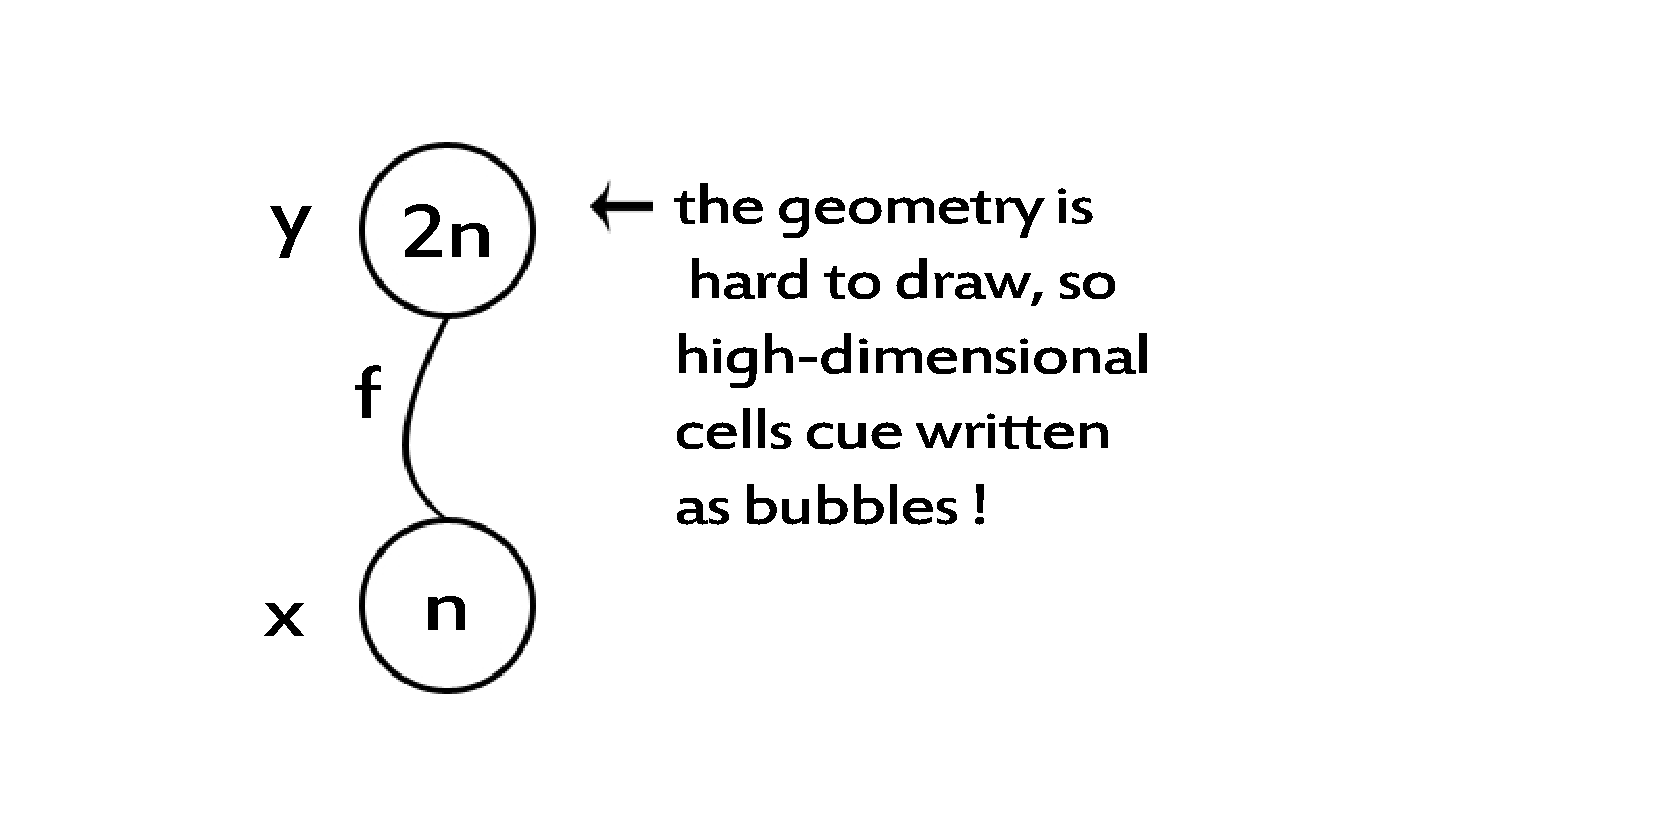
\includegraphics[width=0.3\textwidth]{figures/11.pdf}
\caption{\small Cell diagram of $C(f)$.}
\end{wrapfigure}
Now that we've learned some facts about the squares, we're in a position to apply them to some of the problems that came up earlier.  First, recall that the Hopf invariant $H: \pi_{2n-1} S^n \to \Z$ is defined as follows. $H(f)$ is to be the unique integer (up to sign) for which $x^2=H(f)y$, where $x$ and $y$ are the generators of $H^n(C(f))$ and $H^{2n}(C(f))$ repectively.\footnote{Note that $C(f)$, the cofiber of $S^{2n-1} \stackrel{f}{\to} S^n$ has three cells, one in dimension $0$, $n$ and $2n$.} In particular, $x^2 = H(f) \cdot y \equiv \Sq^n x$ (mod two), so that $H(f)$ is odd iff $\Sq^nx\neq0$.  However, if $n \ne 2^i$, then $\Sq^n$ is decomposable in terms of lower squares, and $\Sq^n x = 0$ since there's no cohomology between $x$ and $y$.  Therefore, we get
\begin{thm}[Adem\footnote{He realized as soon as he got the relations that this was a consequence.}]
If there is an element of odd Hopf invariant on $S^n$, then $n$ is a power of two.
\end{thm}
%\begin{wrapfigure}{r}{0.3\textwidth}
%\centering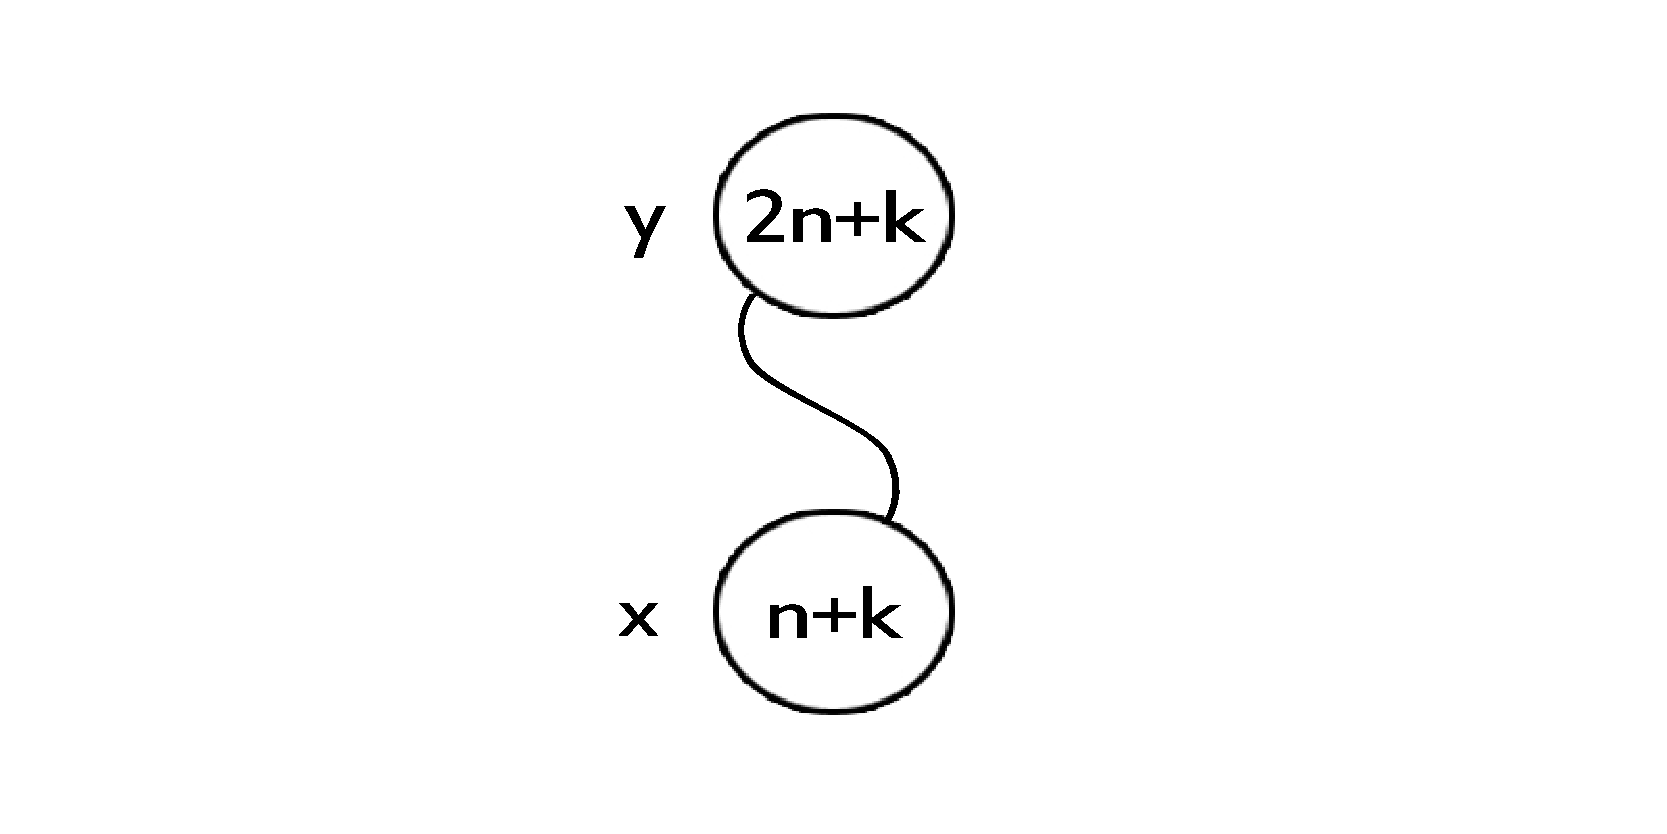
\includegraphics[width=0.3\textwidth]{figures/12.pdf}
%\caption{\small Diagram of $C(g)$.} % this figure should be some kind of staircase of suspensions to see what's going on
%\end{wrapfigure}
Now if $g$ is any map $S^{2n+k-1} \stackrel{g}{\to} S^{n+k} \to C(g)$, then we no longer have a nontrivial cup-product, but we still have $\Sq^n$, so we can define a generalized Hopf invariant $\widetilde H(g)$ by $\Sq^n x = \widetilde H(g) y$, giving $\widetilde H: \pi_{2n+k-1}S^{n+k} \to \Z_2$.  The fact that $\Sq^n$ commutes with suspensions means
\begin{diagram}[height=2em]
f & & \pi_{2n-1} S^n & \rTo^H & \Z \\
\dMapsto & & \dTo & & \dTo \\
\Sigma^k f & & \pi_{2n+k-1} S^{n+k} & \rTo^{\widetilde H} & \Z_2
\end{diagram}
commutes.  $\pi_{2n+k-1} S^{n+k}$ is independent of $k$ for $k \ge 1$; in other words we have turned the unstable question into a related stable one.

Recall next another fact we had, more directly related to the vector field problem: if $S^{n-1}$ has $(k-1)$ everywhere linearly independent vector fields, then $nL \onto \RP^{k-1}$ is fiber homotopy trivial, and this in turn implies the existence of a ``coreduction''
\begin{diagram}[height=2em]
T(nL\downarrow\RP^{k-1}) & \,\cong & \Sigma^n \RP^{k-1}_+ & \rTo & S^n \\
\uTo & & & \ruTo(4,2)_\simeq &  \\
S^n
\end{diagram}
Now we're in a position to study, using the squares, the question of when we can split off the $S^n$ from $T(nL)$.  Remember that we found
\[
T(nL\downarrow\RP^{k-1}) = \RP^{n+k-1}/\RP^{n-1} =: \RP^{n+k-1}_n
,\]
called ``stunted projective space''.  Its mod 2 cohomology is $\widetilde H^*(\RP^{n+k-1}_n) = \langle x^n, x^{n+1}, \ldots, x^{n+k-1} \rangle$, where $|x^i| = i$, and it comes in an obvious way from the cohomology of $\RP^{n+k-1}$.  Now the coreduction above implies that the class $x^n$ in $\widetilde H^n \RP^{n+k-1}_n$ pulls back from the generator of $\widetilde H^n S^n$.  Thus $\Sq^i$ for $i > 0$ is trivial on $x^n$ since it is on $S^n$. That is, $\Sq x^n=x^n$.  Now $x \in \widetilde H^1 \RP^{n+k-1}$ is a 1-dimensional class, so $\Sq x = x + x^2 = x(1+x)$, and as $\Sq$ is a homomorphism, $\Sq x^n = x^n(1+x)^n$. %and we have shown that the fiber homotopy triviality of $nL \onto \RP^{k-1}$ implies that we've calculated this same square another way:
\[
\Sq x^n = x^n(1 + x)^n = x^n
,\]
which implies that $(1+x)^n \equiv 1 \pmod{x^k}$.  Write $n = \sum_{i \in I} 2^i$, a sum of distinct powers $i \in I$ of 2.  Then $\nu(n)$ is the smallest $i$ occuring in $I$ (where $n=\textup{odd}\cdot2^{\nu(n)}$ as above), and
\[
(1+x)^n = \prod_{i \in I} (1 + x)^{2^i} = \prod_{i \in I} (1 + x^{2^i}) = 1 + x^{2^\nu} + \hbox{higher powers}
.\]
That $(1 + x)^n \equiv 1 \pmod{x^k}$ implies that $2^\nu \ge k$.  Recall that our goal is to show that $\rho(n) - 1$, the number of linearly independent vector fields on $S^{n-1}$ which we constructed using Clifford algebras, is equal to the actual number of linearly independent vector fields on $S^{n-1}$ by bounding it above.  Here's a table of $\nu(n)$, $2^{\nu(n)}$, and $\rho(n)$ for some small $\nu(n)$:
\[
\begin{array}{c|cccccc}
\nu(n) & 0 & 1 & 2 & 3 & 4 & 5 \\
\hline
2^{\nu(n)} & 1 & 2 & 4 & 8 & 16 & 32 \\
\hline
\rho(n) & 1 & 2 & 4 & 8 & 9 & 10.
\end{array}
\]
For $\nu(n) \le 3$, then, we have obtained an exact answer, but asymptotically, we're doing pretty badly.

There's another approach to this sort of calculation with Thom spaces and squares.  Suppose that $E$ is an $S^{n-1}$-bundle over a base $B$, which we will always assume to be connected. There is an inclusion into the fiberwise mapping cone $C_B E$, a disk bundle:
\[\xymatrix@R=.6cm{
S^{n-1}\ar[r]&E\,\ar@{^{(}->}[r]\ar[d]&C_BE\ar[d]&D^n\ar[l]\\
&B\ar@{=}[r]&B
}\]
and $T(E) = C_B E / E$.  So $\widetilde H^* (T(E)) = H^*(C_B E, E)$.  Now we can use the relative Serre spectral sequence to get a spectral sequence
\[
E_2^{s,t}=H^s(B, \{H^t(D^n, S^{n-1})\}) \Rightarrow \widetilde H^{s+t}( T(E))
.\]
But this spectral sequence has $E_2^{s,t}\neq0$ only when $t=n$, so that that everything collapses by the $E_2$ page, and we obtain isomorphisms $H^*(B, \{H^n(D^n, S^{n-1})\}) \cong \widetilde H^{*+n} (T(E))$.  In general $B$ is not simply connected, so we need twisted coefficients.  If the system of local coefficients is trivial, then this isomorphism is the Thom isomorphism.  An orientation of $E$ is then just that: a choice of trivialization of this local coefficient system.

Working over $\Z_2$ coefficients, this coefficient system is already canonically trivial, so the concern about orientation doesn't mean anything, and we get $H^*(B; \Z_2) \cong \widetilde H^{*+n} (T(E))$ anyway.  For example, in the case of $nL \onto \RP^{k-1}$ we see trivially that the isomorphism comes from multiplication by $x^n$.  This comes out in general from the multiplicative structure of the spectral sequence, as follows.

First, $1\in H^0 (B)$ corresponds under the Thom isomorphism to some $u \in \widetilde H^n (T(E))$, called the ``Thom class''.  Now $\widetilde H^* (T(E)) = H^*(C_B E, E)$ is a module over $H^* (B)$ via the ``cup product'' pairing, the composite:
\[\xymatrix{
H^*(B) \otimes H^*(C_B E, E)\ar[r]^{p^*\otimes1\ \ \ }&H^*(C_B E) \otimes H^*(C_B E, E)\ar[r]^{\hspace{9mm}\smile}& H^*(C_B E, E)
}\]
We justify calling this a cup product as $p^*$ is an isomorphism, as $C_BE$ is a disk bundle, so we can almost ignore the ``pulling back'' part of the operation. The Thom isomorphism says that cup-product by the Thom class $u$ is an isomorphism $\smile u: H^* (B) \cong \widetilde H^* (T(E))$.

This enables us to talk about $\widetilde H^* (T(E))$ without much reference to $T(E)$ beyond the Thom class.  For example, suppose we wished to calculate $\Sq y$ for some $y\in \widetilde H^*( T(E))$. Now $y=xu = x \smile u$, for some unique $x \in H^* B$, and $\Sq y = (\Sq x)(\Sq u)$ by the Cartan formula, so all we need to know is $\Sq u$.  Again using the Thom isomorphism, we write $\Sq^k u = w_k u$, where $w_k \in H^k B$. We call $w_k = w_k(E)$ the ``$k$th Stiefel-Whitney class of $E$'', and we write $w = \sum_{k \ge 0} w_k$, the ``total Stiefel-Whitney class of $E$''.

Of course, if $V$ is a vector bundle, we write $w(V)$ for $w(S(V))$. The following facts follow immediately:
\begin{itemize}
\item $w_k$ depends only on the fiber homotopy type of the sphere bundle.
\item $\Sq^0 u = u$, so $w_0 = 1$.
\item $w_k = 0$ for $k > n$.
\item External Whitney sum formula:\footnote{Whitney says this is the hardest theorem he ever proved, but he had the wrong definition of Stiefel-Whitney classes.} $w(E'\mathop{\widehat\ast}E''\downarrow B'\times B'')=w(E'\downarrow B')\times w(E''\downarrow B'')$ for sphere bundles $E'\downarrow B'$ and $E''\downarrow B''$.
\item Internal Whitney sum formula: $w(E'\mathop{\ast_B} E''\downarrow B)=w((E'\downarrow B)\smile w(E''\downarrow B))$ for sphere bundles $E'\downarrow B$ and $E''\downarrow B$.
In particular, $w(V'\oplus V'')=w(V')\smile w(V'')$ for vector bundles $V',V''$ over $B$.
\item Stability: One calculates $w(n\varepsilon) = 1$, so that $w(V \oplus n\epsilon) = w(V)$  (using the Whitney sum formula).
\end{itemize}
\begin{lem}\label{ThomClassLem}
Suppose that $E\downarrow B$ is an $S^{n-1}$-bundle over a connected base, and that $s:S^n\to T(E)$ is the inclusion of copy of $S^n$ over the basepoint, and that $u\in H^n(T(E))$ is the Thom class. Then $s^*(u)$ is the generator $\mathit{o}\in H^n(S^n)$ that corresponds to the standard orientation\footnote{That is, the orientation on $S^n=(D^n,S^{n-1})$ which was used to trivialise the coefficient system used in the Serre spectral sequence which provided the Thom isomorphism.} of $S^n$.
%Alternatively, $u$ is the class dual to $s_*(S^n)\in H_n(T(E))$.
\end{lem}
\begin{proof}
This follows by naturality of the Thom isomorphism for oriented maps of oriented $S^{n-1}$-bundles, once it has been checked for the trivial $S^{n-1}$-bundle $\mathcal{E}=S^{n-1}\downarrow*$ (a simple task). Consider the map of oriented $S^{n-1}$-bundles (shown at left):
\[\xymatrix{
\mathcal{E}\ar[r]\ar[d]&E\ar[d]\\
\ast\ar[r]&B
}\qquad\qquad\qquad\qquad
{
\xymatrix{
\makebox[0mm][r]{$S^n=\,$}T(\mathcal{E})\ar[r]&T(E)\\
S^n\ar@{=}[u]\ar[ur]
}\qquad\qquad\qquad
\xymatrix{
u_\mathcal{E}\ar@{=}[d]&\ar@{|->}[l]u_E\ar@{|->}[dl]\\
\mathit{o}
}}\]
This map induces the commuting diagram in the middle: a map of Thom spaces relative to $S^n$. Using this commuting diagram, we can calculate $s^*(u_E)$ in two different ways (at right) to obtain the result.
\end{proof}
\begin{proof}[Proof of Whitney sum formula]
 Let $E' \downarrow B'$ be an $S^{n-1}$-bundle and $E'' \downarrow B''$ be a $S^{m-1}$-bundle; let $E\downarrow B$ be the fiberwise join, an $S^{m+n-1}$-bundle.  Now, $T(E) = T(E') \sprod T(E'')$, and moreover, $u = u' \sprod u''$. To see this, recall that the inclusion $S^{n+m}\hookrightarrow T(E)$ is the wedge of the inclusions $S^{n}\hookrightarrow T(E')$ and $S^{m}\hookrightarrow T(E'')$. Now by the characterisation of $u$ in lemma \ref{ThomClassLem}, we see that $u$ pulls back to the orientation generator in $H^{n+m}(S^n\wedge S^m)$, which is the wedge of the orientation generators in $H^n(S^n)$ and $H^m(S^m)$.

Thus, $\Sq u = \Sq(u' \sprod u'') = \Sq u' \sprod \Sq u''$. Note that the first expression models $w(E) \smile u$, while the third expression models $w(E') \sprod w(E'') \smile u' \sprod u''$.  Therefore, $w(E) = w(E') \sprod w(E'')$.
\end{proof}

Now the Thom class of $nL \onto \RP^{k-1}$, as we saw, is $x^n$.  So $w(L) = 1 + x$, and $w(nL) = (1+x)^n$.  So $nL \onto \RP^{k-1}$ is fiber homotopy trivial only if $(1+x)^n \equiv 1 \pmod{x^k}$, which is the same result we obtained before.  Now the program is to improve the results by pursuing a similar set of results in $KO$-theory.

% >>>
\fi
\BoxedNote{
\Bullet Using the decomposability of $\Sq^i$ for $i\neq2^j$, there can only be an element of Hopf invariant one in $\pi_{2n-1}(S^n)$ if $n=2^j$.

\Bullet $\Sq x^n=x^n(1+x)^n$, where $x^n\in\widetilde H^n(\RP^{n+k-1}_n)$. If there is a coreduction, then $\Sq x^n$ must equal $x^n$. Thus, a necessary condition for $k-1$ fields on $S^{n-1}$ is that $(1+x)^n\equiv 1$ in $\Z_2[x]/(x^k)$, which implies $2^{\nu(n)}\geq k$.

\Bullet For an oriented $S^{n-1}$-bundle $E$, $\widetilde H^*(T(E))$ is an $H^*(B)$-module under ``$\smile$'':
\[\xymatrix{H^*(B) \otimes H^*(C_B E, E)\ar[r]^{p^*\otimes1\ \ \ }&H^*(C_B E) \otimes H^*(C_B E, E)\ar[r]^{\hspace{9mm}\smile}& H^*(C_B E, E)}\]
Defined the Thom class $u\in H^n(T(E))$ such that $\smile u$ is the Thom isomorphism $H^*(B)\to\widetilde H^{*+n}(T(E))$.

\Bullet The Stiefel-Whitney classes $w_i(E)\in H^i(B)$ are defined by $w(E)\smile u=\Sq u$. They vanish for $i>n$, and $w_0=1$. They satisfy the Whitney sum formula $w(V\oplus W)=w(V)\smile w(W)$, and are stable: $w(V\oplus \epsilon)=w(V)$.
}
